\documentclass[12pt,a4paper]{amsart}

\usepackage{amsmath}
\usepackage{graphicx}
\usepackage{amsrefs}
\usepackage{parskip}
\setlength{\parskip}{0.8em}

\title{Project Plan}
\author{bmjm501 }
\date{October 2024}

\begin{document}

\maketitle

% \section{Questions}

% THE QUESTIONS I WANT ANSWERS TO:

% 1. why is the study of chaos important in classical systems?

% 2. Why do we quantise the systems to study chaos in quantum mechanics?

% 3. How does chaos happen in iterated maps? (Already got the answer from Schek)

% 4. What classical mechanics is important (talk about Hamiltonian mechanics and then integrable systems, difference between conservative systems and dissapitive systems)

% 5. What are features of chaotic behaviour? (bifucations, perioud doubling)

% 6. What quantifies chaotic behaviour (Lynapov exponent)

\section{Project Context}

\subsection{Talk abit about what chaos is}
My project will delve into topics in the field of \textbf{chaos theory}, particularly in classical and quantum systems. Chaotic systems are a type of non-linear dynamical system that have exhibit behaviours that "appears" random or noisy. However throughout the centuries, universal qualitative and quantitative features of chaotic systems have been discovered, and now chaos theory explains solutions of equations in a large variety of fields such as population dynamics, chemical kinetics and celestial mechanics. [REFERENCE CHAOS] 

As we are concerned with dynamical systems, initial conditions of a state of the system and the evolution of a solution to the equations that govern the system, or a trajectory, become fundamental concepts to utilise. A trajectory can evolve with any rule the dynamical system dictates, the simplest one being evolution with time.

\subsection{Iterated Map example}

An example of dynamical systems are iterated maps, which have form $x_{i+1} = f(x_{i})$. These are important as the can be used to model more complex systems and give us useful insights as to how these trajectories of the system evolve by studying each iteration of the map. REFERENCE PG 180 OF HILBORN.

Consider the closed mapping $$x_{i+1} = {\mu} x_{i} (1 - x_{i}) \equiv f(\mu, x_{i})$$ on the unit interval $x_{i} \in [0, 1] \  {\forall}i \in \mathbb{N}$. This is called \textit{the logistic equation}, which can be used for biological models such as population growth [REFERENCE HILBORN]. The value $\mu$ is a control parameter. An important concept in these systems is to define the fixed points of the map i.e. a point $x^{*}$ such that $x^{*} = f(\mu, x^{*})$. For this mapping, the fixed points are $$x^{*} = 0 \quad x^{*} = 1 - \frac{1}{\mu}$$ A fixed point has an associated stability, which can be found by analysing the absolute value of the derivative of the function $f(\mu, x)$ evaluated at a given fixed point. A stable or attracting fixed point is such that $|f'(x^{*})| < 1$ and iterations $x_{1} \rightarrow x_{2} \rightarrow \cdots \rightarrow x^{*}$ converge to the fixed point (like the trajectories are "attracted" to the point). Considering the non-trivial fixed point of the logistic equation, $|f'(\mu, x^{*})| = |2 - \mu|$ which gives restrictions on the value of $\mu$. Notably, $\mu \leq 4$ so that the mapping remains closed under the interval and the fixed point $x^{*}$ is stable for $1 < \mu < 3$. However when $\mu > 3$, the trajectories now oscillate between two points, which can be labelled $x_{1}^{*}$ and $x_{2}^{*}$, and the mapping undergoes a bifurcation as described earlier. This behaviour is studied by considering the composition $f \circ f$ of the original mapping. Now $x_{1}^{*}$ and $x_{2}^{*}$ are fixed points of the composition of the map. As $\mu$ increases, this splitting of trajectories occurs more and more often, leading to the bifurcation diagram shown in Figure \ref{fig:bif}.

\begin{figure}[h] 
    \centering
    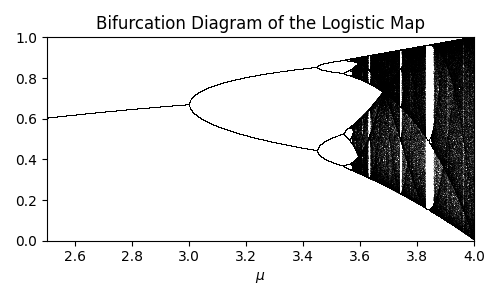
\includegraphics[scale=0.8]{logistic_map_bifur.png}
    \caption{A bifurcation diagram for the logistic map, for varying $\mu$ values. The first splitting occurs at $\mu$ = 3 as described.}
    \label{fig:bif}
\end{figure}


\subsection{Hamiltonian Mechanics}

The foundations of classical chaos lie in Hamiltonian mechanics. Importantly, the study of \textit{Hamiltonian} or \textit{conservative} systems rather than dissipative systems like ones described by the logistic map. Hamiltonian systems evolve by Hamilton's equations, famously:
$$\dot{q}_{i} = \frac{\partial \mathcal{H}}{\partial p_{i}} \quad \dot{p}_{i} = -\frac{\partial \mathcal{H}}{\partial q_{i}} \quad i = 1, \cdots , N$$
for generalised coordinates $q_{i}(t)$, generalised momenta $p_{i}(t)$ and $N$ degrees of freedom. The \textit{phase space} of the system describes the set of solutions (or states) of the system on a $p$ and $q$ axis. The use of phase space is necessary when describing the evolution of a specific trajectory. If a physical quantity remains constant along a trajectory, then it is called a \textit{constant of the motion}. 

These constants can always be defined by a function $J_{i}(q, p)$ [REFERENCE HULBORN PG 323], and each $J_{i}$ can have an associated function $\Theta_{i}(q, p)$. These are usually named the \textit{action} and \textit{angle} variables, and they are chosen such that they follow a canonical transform of $q$ and $p$ i.e:
$$\dot{\Theta}_{i} = \frac{\partial \mathcal{H}}{\partial J_{i}} \quad \dot{J}_{i} = -\frac{\partial \mathcal{H}}{\partial \Theta_{i}}$$
In the case where a canonical transform produces a Hamiltonian such that $\dot{J_{i}} = 0 \ \forall i$, then that system is called \textit{integrable}. An important consequence of this is that there are as many constants of motions as there are degrees of freedom in integrable systems. Thus naturally, a \textit{non-integrable} system has fewer constants of the motions than degrees of freedom. It is these kinds of systems that exhibit chaotic behaviour, and further study is needed into why this is.

 
 PG 334 LEADS ON TO QUANTUM, RIGHT ST END
 PG 328 ABOUT WHERE NON-INTEGRABLE SYSTEMS COME UP


% Consider 
\subsection{Quantisation}

\section{Milestones and Deliverables}



\end{document}
